\chapter{FPGA}
\label{ch:into}

\section{Εισαγωγή}
\begin{frame}
  \frametitle{FPGA}
  \begin{itemize}
    \item FPGA stands for Field Programmable Gate Array.
    \item It is a type of integrated circuit that can be configured by the user after manufacturing.
    \item FPGAs are used in a wide range of applications, including digital signal processing, telecommunications, and automotive systems.
  \end{itemize}
  
\section{Αρχιτεκτονική u200}
\begin{figure}[h!]
  \centering
  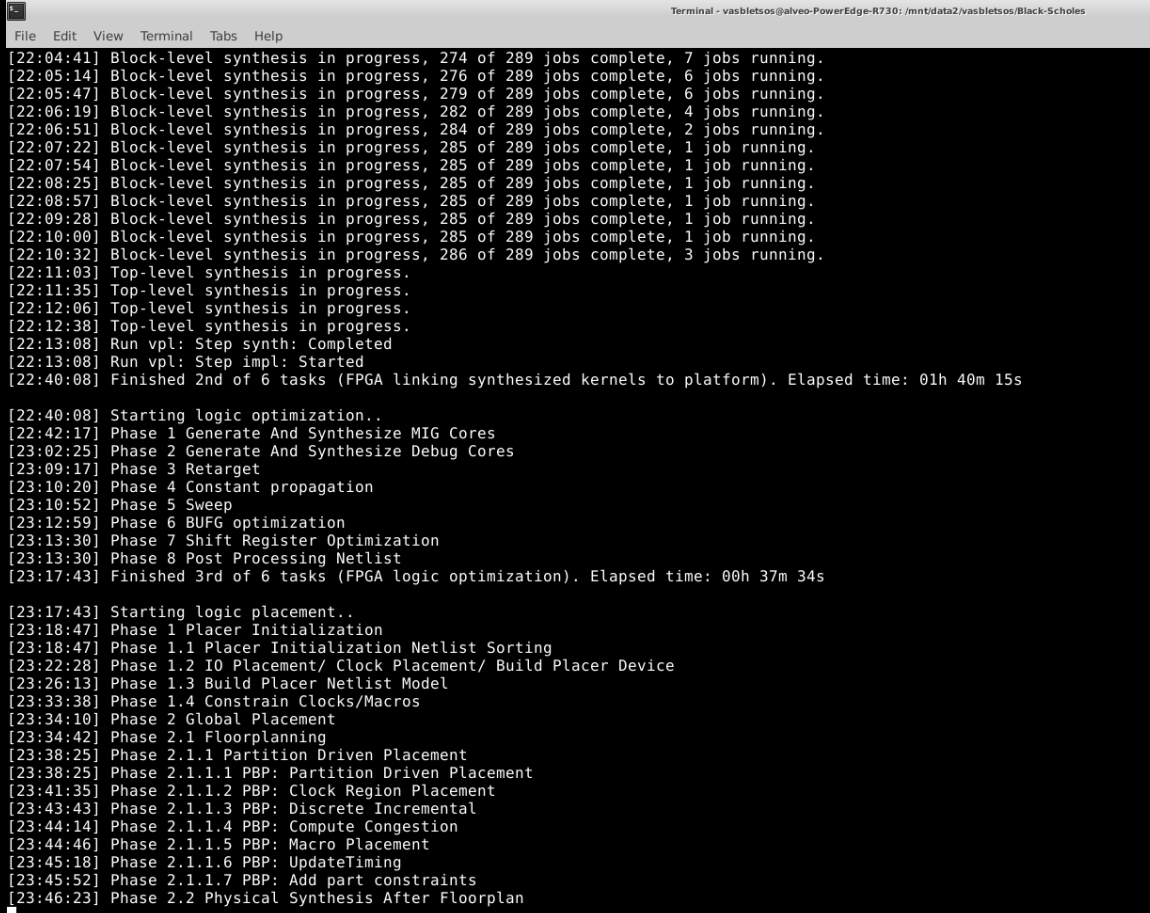
\includegraphics[width=0.8\textwidth]{figures/synthesis.png}
  \caption{FPGA Synthesis}
  \label{fig:hw_synthesis_fpga}
\end{figure}

\section{Variable Types}
\section{Vivado}
\section{Vitis HLS}
\section{Simulation}
\section{Synthesis}